\documentclass[9pt,t]{beamer}
\mode<presentation> {
	\usetheme{Berkeley}
	\usecolortheme{whale}
} 
\usepackage{amsthm, hhline}
\usepackage{stmaryrd, mathtools, stmaryrd}
\usepackage{amsmath, amssymb, graphicx,array}
\usepackage{mathtools}
\DeclareMathOperator{\lcm}{lcm}
\usepackage{booktabs,comment,bbm}
\newcommand{\Z}{\mathbb{Z}}
\newcommand{\N}{\mathbb{N}}
\usepackage[english]{babel}
\usepackage[utf8x]{inputenc}
\usepackage{color}
\usepackage[export]{adjustbox}
\usefonttheme{serif}
\setbeamerfont{title in sidebar}{size=\fontsize{2}{4}\selectfont}
\setbeamerfont{author in sidebar}{size=\fontsize{2}{4}\selectfont}
\setbeamerfont{section in sidebar}{size=\fontsize{2}{4}\selectfont}
\setbeamerfont{subsection in sidebar}{size=\fontsize{2}{4}\selectfont}
\newtheorem{proposition}[theorem]{Proposition}
\fontsize{6pt}{7.2}
\DeclareMathOperator{\ex}{\mathbb{E}}
\DeclareMathOperator{\pr}{\mathbb{P}}
\DeclareMathOperator{\indic}{\mathbbm{1}}
\DeclareMathOperator{\cov}{cov}
\DeclareMathOperator{\var}{var}
\DeclareMathOperator{\sgn}{sgn}
\DeclarePairedDelimiter\ceil{\lceil}{\rceil}
\DeclarePairedDelimiter\floor{\lfloor}{\rfloor}
\DeclarePairedDelimiter\abs{\lvert}{\rvert}


\title{Bernoulli Line Ensembles and the Airy 2 Process}
\author{Xiang Fang, Lukas Fesser, Christian Serio, Carson Teitler, and Angela Wang}
\institute{Columbia University REU}
\date{July 22, 2020}
\begin{document}
	\begin{frame}
		\maketitle
	\end{frame}
\section{Introduction (5-6 min)}
\begin{frame}{Gaussian Universality}
Gaussian universality (CLT, Donsker Theorem)
\begin{figure}
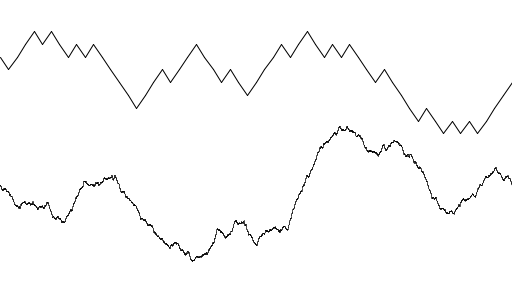
\includegraphics[height=0.5\textheight]{graphics/Gaussian.png}
\caption{An example of a Bernoulli random walk and a Brownian Motion}
\end{figure}

\end{frame}
\begin{frame}{Multple Random Walks}
Increase the number of walkers (avoiding Bernoulli random walks and Dyson BM)
\begin{figure}
	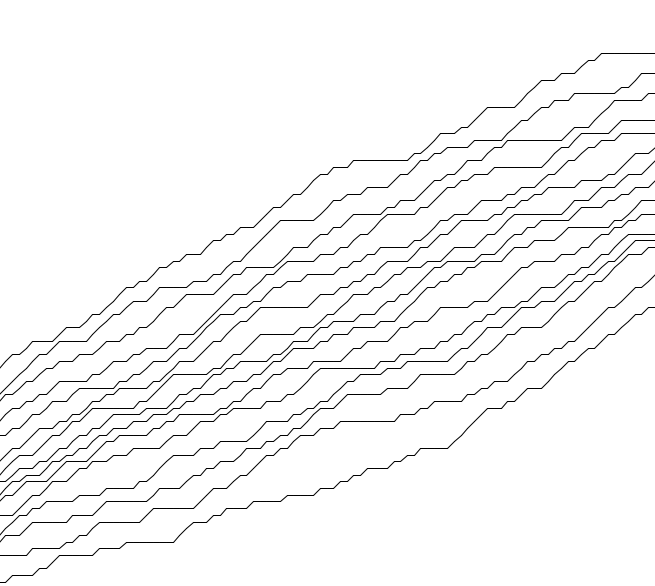
\includegraphics[height=0.5\textheight]{graphics/MultipleBernoulli.png}
	\caption{Multiple Bernoulli Random Walks}
\end{figure}
\end{frame}
\begin{frame}{Airy Line Ensemble}
What happens as N (number of walkers) goes to infinity? new type of limit occurs Airy line ensemble, top curve is the Airy process. Increasing the number of paths pushes us outside of the Gaussian universality class and into what is called the ”KPZ universality class”
\end{frame}
\begin{frame}{Open Question}
Big open problem: Show that for “generic random walks” with “generic” initial conditions we have convergence to Airy LE. This problem is open even for Bernoulli random walks (only known if all are started from 0)
\end{frame}

\section{Convergence to Airy Line Ensemble (6-7 min)}
\begin{frame}{How to show this?}
Finite dimensional convergence (very hard, algebraic need good formulas)
Show tightness (i.e. existence of weak subsequent limits) -- easier, qualitative/analysis. You need to control min, max, modulus of continuity
\begin{figure}
	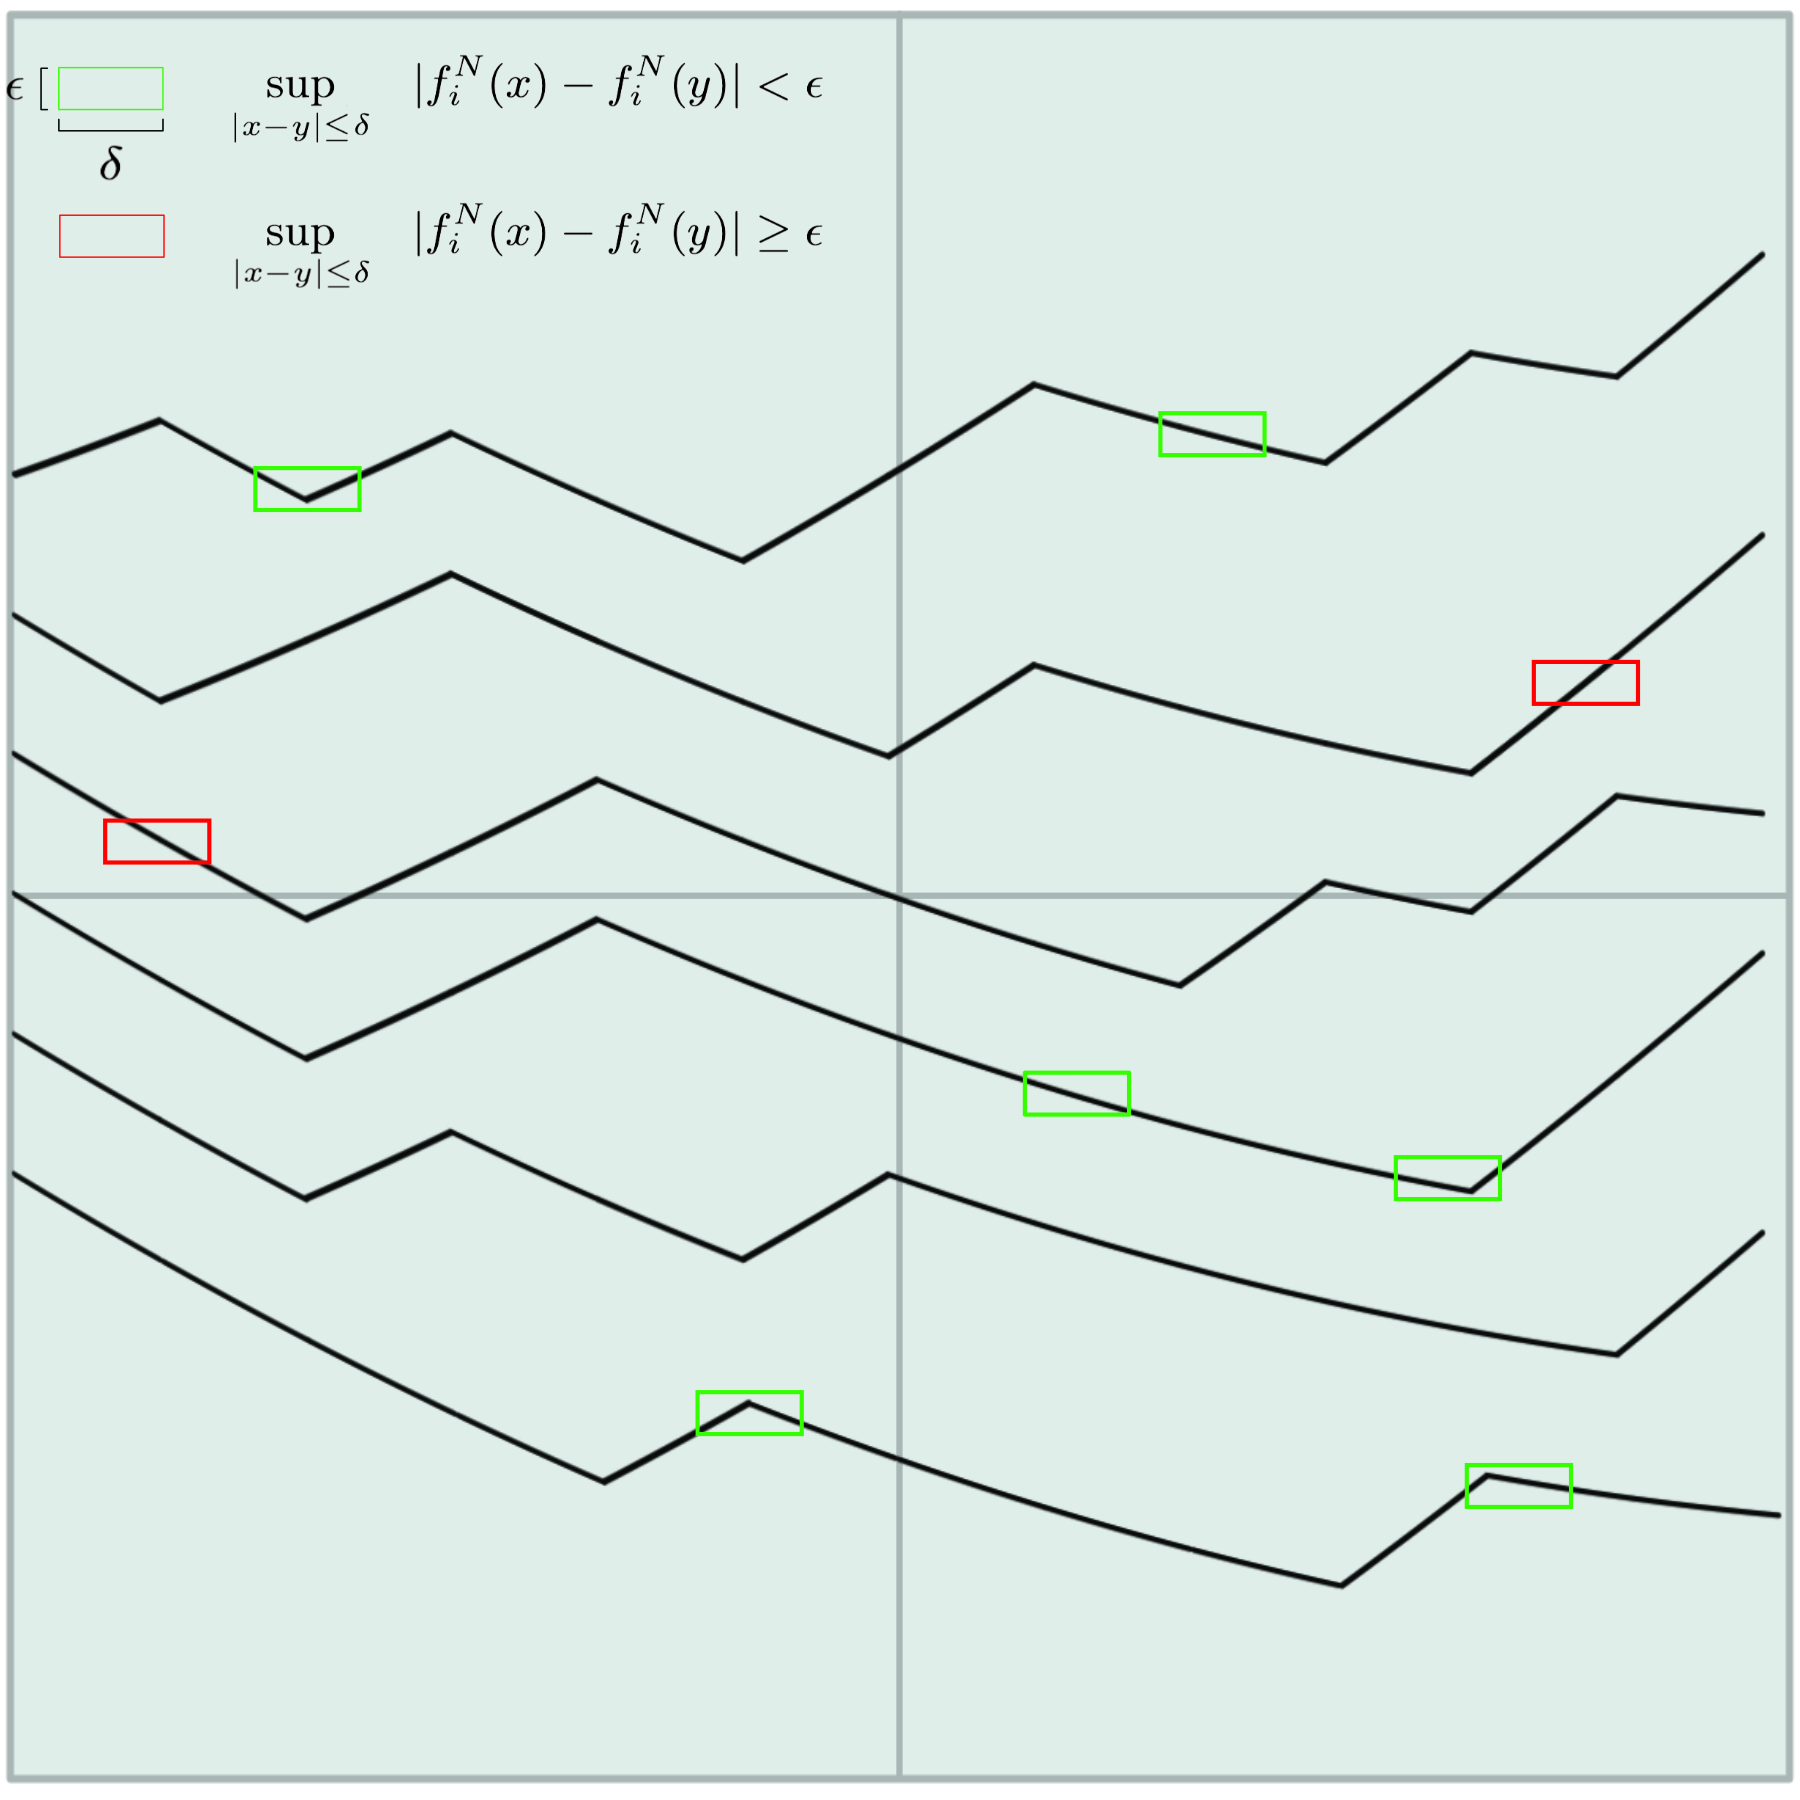
\includegraphics[height=0.5\textheight]{graphics/TempModulusCont.jpg}
	\caption{The Modulus of Continuity}
\end{figure}

\end{frame}
\begin{frame}{Our Result}
Main result here: if top line 1 point marginals at integer times go to Tracy-Widom then the full LE is tight. 
$P(L_1(nN^{2/3}) - nN^{2/3} p + \lambda n^2 N^{1/3} \leq N^{1/3} x) \to F_{TW}(x)$
\end{frame}
\begin{frame}{Previous Results}
Compare to Virag+Duavergne+Nica ‘19 (they assume fd convergence to Airy Line ensemble vs we assume only 1 point convergence of the top line to TW)
\end{frame}
\section{Section of Paper (7-9 min)}
\begin{frame}
Arguments are inspired by [Corwin-Hammond ‘14, ‘15] (continuous setting) [Corwin-Dimitrov ‘17] (discrete setting) Description of the problem ( min, max and modulus of continuity)
2 min   $P( \max_{[-r, r]} L_1(sN^{2/3}) - psN^{2/3}  > RN^{1/3} ) < \epsilon$ if $R$ is large enough  
\end{frame}
\begin{frame}
Proof  (mention monotone coupling lemmas somewhere ) - say MC with picture
2min
\end{frame}
\begin{frame}
Proof  (mention strong coupling somewhere) - say SC with picture 
L = Bernoulli bridge B is a Brownian bridge with variance. There is a probability space such that $P( sup \abs*{L - B} \geq k (\log N)^2) < \epsilon$. This is a comparison that allows for example to compare the modulus of continuity of the two. [Dimitrov-Wu ‘19]
2 min
\end{frame}
\begin{frame}
Remind: 1. Max on [r, R] and [-R, r] does not deteriorate. 2. Monotone coupling lemmas show that min [-r, r] does not dip to -infty -- this controls min. 
2 min 
\end{frame}
\begin{frame}
(if you have time) In the last (-1 min) we can say a few words about why the max on [r,R] does not deteriorate -- utilizes built in convexity of the problem. Focus on 2 lines 
$P(L_1(nN^{2/3}) - nN^{2/3} p + \lambda n^2 N^{1/3} \leq N^{1/3} x) -> F_{TW}(x)$ - emphasize the parabolic shift
\end{frame}
\end{document}